\sectionmark{Zusammenhänge AF u. Architektur}
\label{sec:anwendungsfaelle}

\textbf{Autor: Torben, Arbnor} 

In diesem Abschnitt behandeln wir unsere zuvor erstellten Anwendungsfälle, indem wir die dazugehörigen Sequenzdiagramme erstellen und diese beschreiben. Dabei wird aufgezeigt, wie der Nachrichtenverkehr zwischen allen im Anwendungsfall beteiligten Modulen abläuft.

Bei der Erstellung der folgenden Sequenzdiagramme haben wir die Software Quick Sequence Diagramm Editor verwendet. Wir haben uns für die Notation an die im Rahmen der Softwareprojekt 1-Vorlesung und Tutorium vorgestellten Notation gehalten und können in den Vorlesungsfolien von Prof.Dr.Rainer Koschke zu Softwareprojekt 1 im Sommersemester 2017 eingesehen werden.

\subsection{Anwendungsfall D1: Login als Prüfling}
Der Prüfling ruft die Webseite auf, die per Default unsere  \texttt {Index.html} ist, auf den der Benutzer seinen Usernamen und das Passwort setzten kann. Zunächst wird über index.xhtml über getLanguage() die Sprache geholt. Danach wird zunächst ein neues  \texttt {LoginBean} instanziiert, mit der davor instanziierten  \texttt {Session} und der dazugehörigen  \texttt {UserDAO}. Für den Loginwerden die Methoden setUsername() und setPassword() aus der  \texttt {LoginBean} Klasse aufgerufen. Per Klick auf den Button "Einloggen", wird in der  \texttt {LoginBean} die Methode login aufgerufen, die zunächst abgfragt, ob der Benutzer überhaupt schon eingeloggt ist. Da der Benutzer noch nicht eingeloggt ist, wird False zurückgegeben. In der Annahme, dass der Benutzer nicht null ist, wird letztendlich der String  \texttt {dashboard.xhtml}zurückgegeben, das dazu führt, dass der  \texttt {User} sich nach erfolgreichem Login direkt auf seinem Dashboard befindet.

\begin{figure}[H]
	\centering
	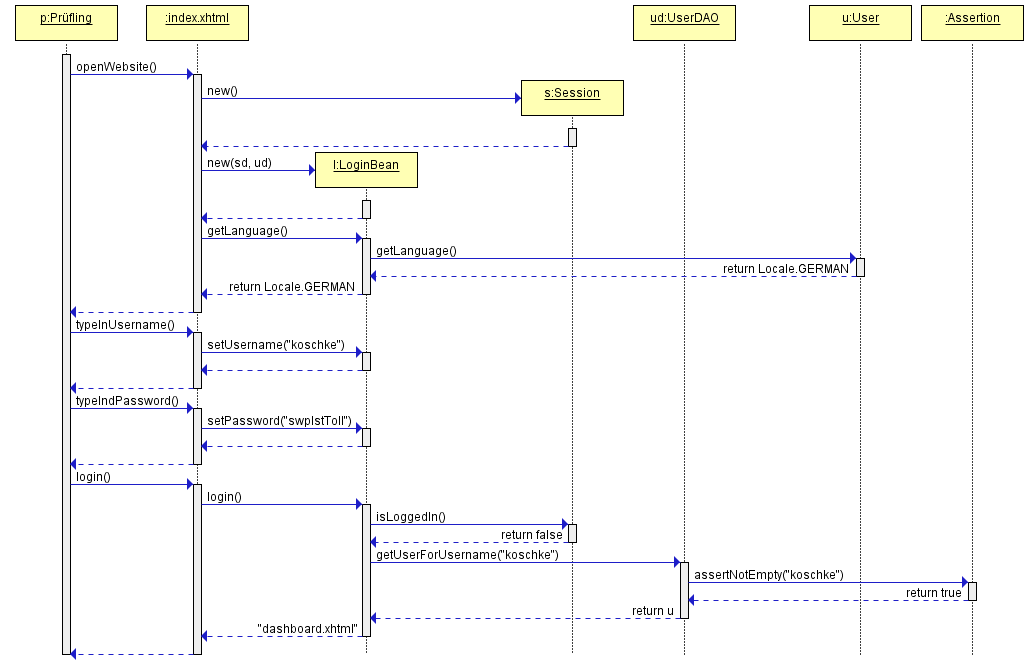
\includegraphics[width=\textwidth,height=15cm,keepaspectratio]{../UMLDiagramme/d1_login}
	\caption{Anwendungsfall D1 : Login als Prüfling}
	\label{fig1}
\end{figure}



\subsection{Anwendungsfall D55: Passwort-Vergessen-Funktion}
Bis zu dem Punkt das eine neue \texttt {LoginBean} instanziiert wird, läuft dieser Sequenzdiagramm gleich, wie das zuvor vorgestellte Diagramm, ab.
Über die  forgotPassword() wird aus der index.html eine neue \texttt {ForgotPasswordBean} instanziiert mit der Session und der MessageDao als Parameter. Dafür wird zunächst die zum Passwort zugehörige Email vom Benutzer in der GUI eingetippt. Mittels setEmail aus \texttt {ForgotPasswordBean}, die aus der \texttt {index.html}  aufgerufen wird, wird die Email gesetzt.
Außerdem wird über die GUI die Martikelnummer vom Benutzer eingetippt und mittels setMatrNr() über \texttt {ForgotPasswordBean} gesetzt.

Sobald die erforderlichen Daten eingetippt und gesetzt sind, kann über den sendPassword-Button in der GUI, welcher sendPassword aus \texttt {ForgotPasswordBean} aufruft, geklickt werden. Dabei verhält sich sendPassword folgendermaßen.
Aus der \texttt {UserDAO} wird mit der übergebenen Email der User aus der Datenbank geladen, und zwar mittels Methodenaufruf getUserForEmail(). Danach wird für den geladenen User mittels getPassword() das Passwort geladen. Damit haben wir alle benötigten Informationen, die wir dem User als Nachricht zusenden können.

Also wird eine neue Nachricht instanziiert, wobei der Empfänger, der Inhalt und der Betreff  durch die \texttt {ForgotPasswordBean} im \texttt {Message}-Objekt gesetzt werden.
Schließlich wird die Nachricht  mittels send() versendet, und mittels save() gespeichert. Schlussendlich wird ein String zurückgegeben, dass die Nachricht versendet wurde. In unserem Fall lautet die Nachricht "Passwort wurde versendet".

\begin{figure}[H]
	\centering
	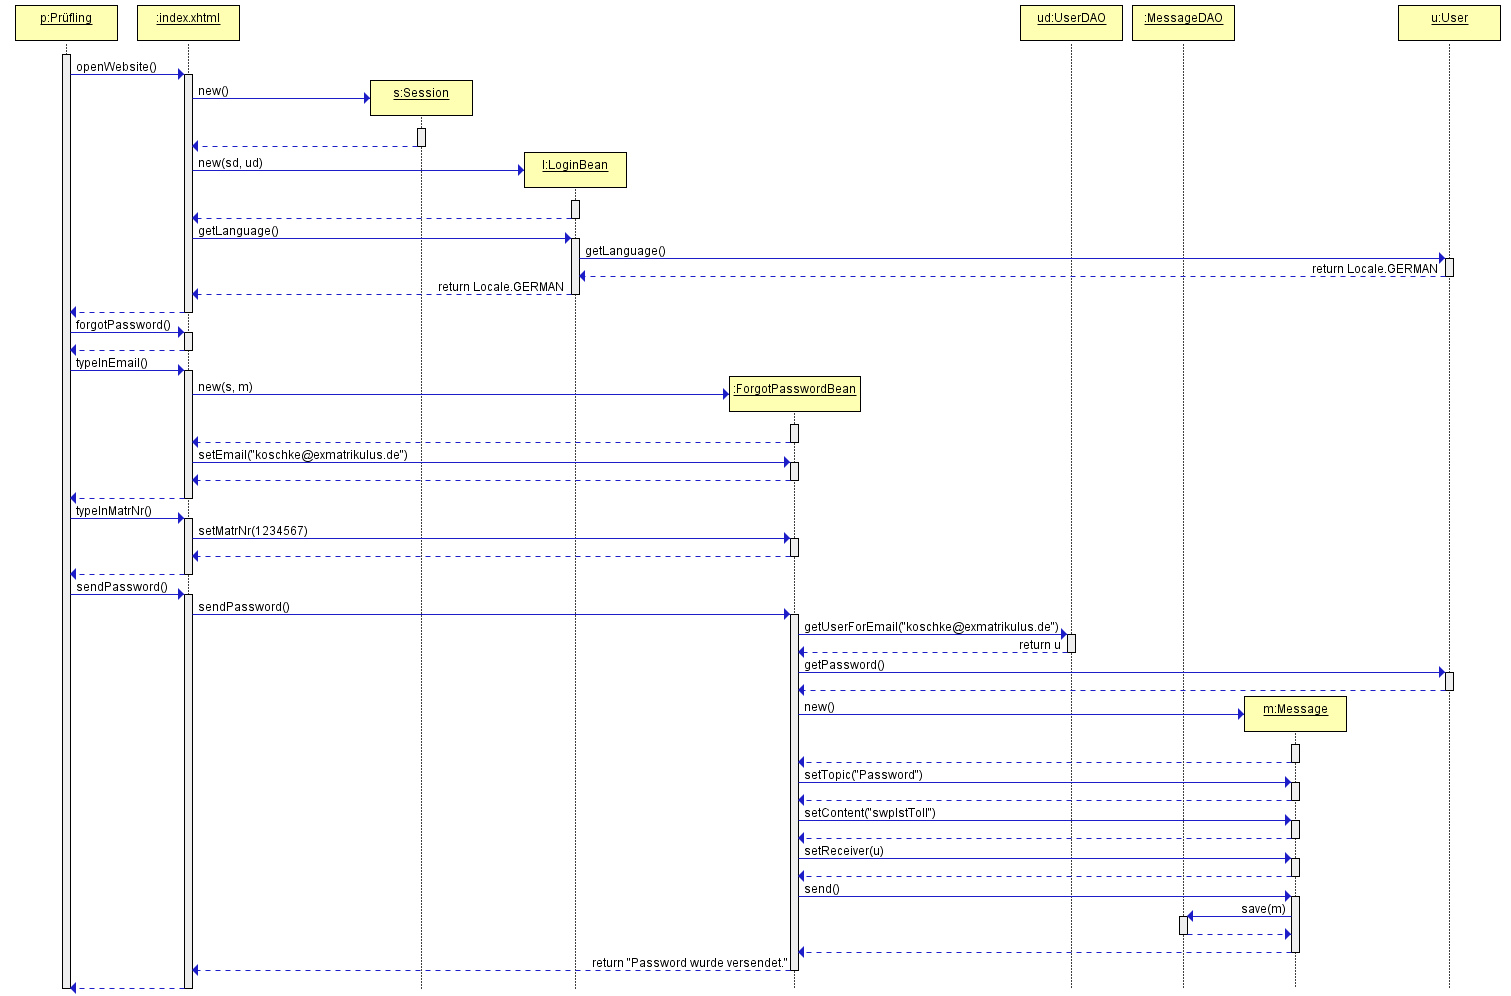
\includegraphics[width=\textwidth,height=15cm,keepaspectratio]{../UMLDiagramme/d55_forgotPassword.png}
	\caption{Anwendungsfall D55 : Passwort-Vergessen-Funktion}
	\label{fig1}
\end{figure}


\subsection{Anwendungsfall D24: Prüfungstermin festlegen}

Über die GUI wird eine neue Prüfung für die Lehrveranstaltung erstellt, die über die Bean \texttt {LectureInstanceExamBean} gesteuert wird. Bei der Erstellung einer neuen Prüfung wird ein neues Objekt vom Typ \texttt {Exam} erstellt, dabei werden alle benötigten Attribute gesetzt, wie dem Datum, der Länge, den Prüfer usw.
Am Ende wird das neue Objekt (die Prüfung) in der DAO über save abgespeichert und die ILV wird geupdated. 


\begin{figure}[H]
	\centering
	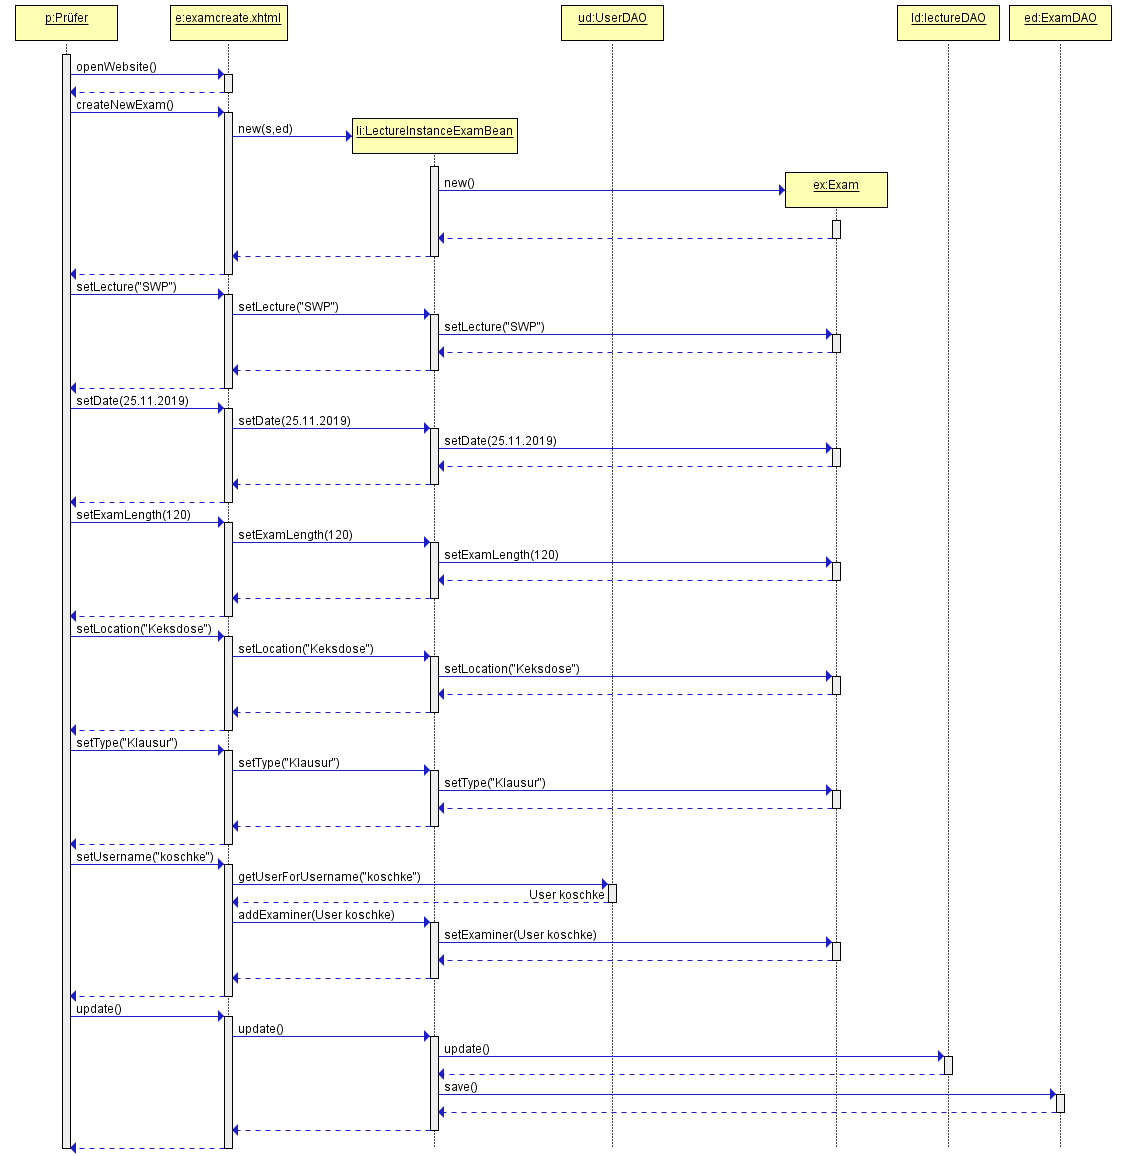
\includegraphics[width=\textwidth,height=15cm,keepaspectratio]{../UMLDiagramme/d24_pruefungstermineFestlegen.png}
	\caption{Anwendungsfall D24 : Prüfungstermin festlegen}
	\label{fig1}
\end{figure}





